\begin{figure}[!tbp]
  \centering
  \begin{minipage}[b]{1\textwidth}
  	\centering
  	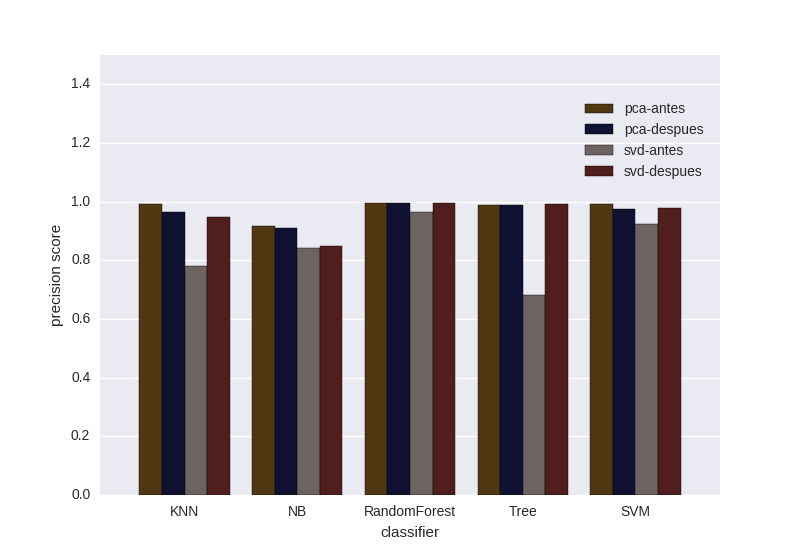
\includegraphics[width=1\textwidth]{../results/precision.png}
    \caption{Medida de performance de los distintos clasificadores utilizando precision-score.}
	\label{figure:precision}
  \end{minipage}
  \hfill
  \begin{minipage}[b]{1\textwidth}
  	\centering
	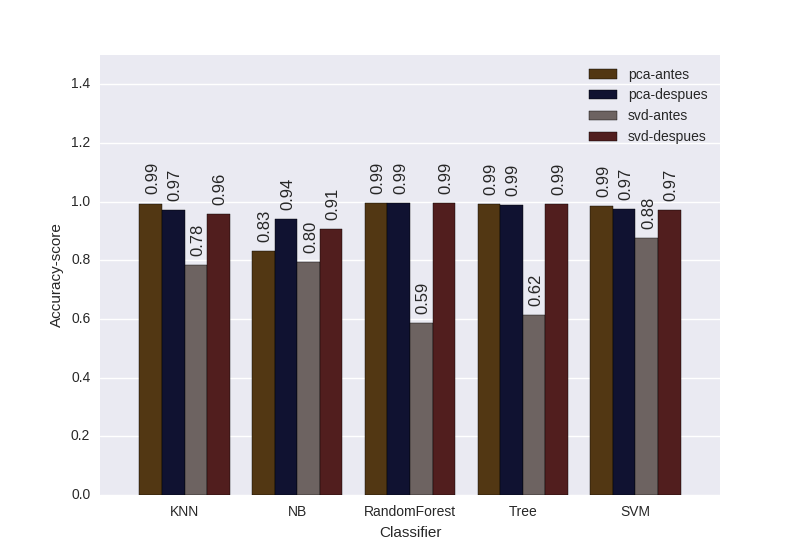
\includegraphics[width=1\textwidth]{../results/accuracy.png}
    \caption{Medida de performance de los distintos clasificadores utilizando precision-score.}
	\label{figure:accuracy}  
  \end{minipage}
\end{figure}

\begin{figure}[h!]
	\centering
	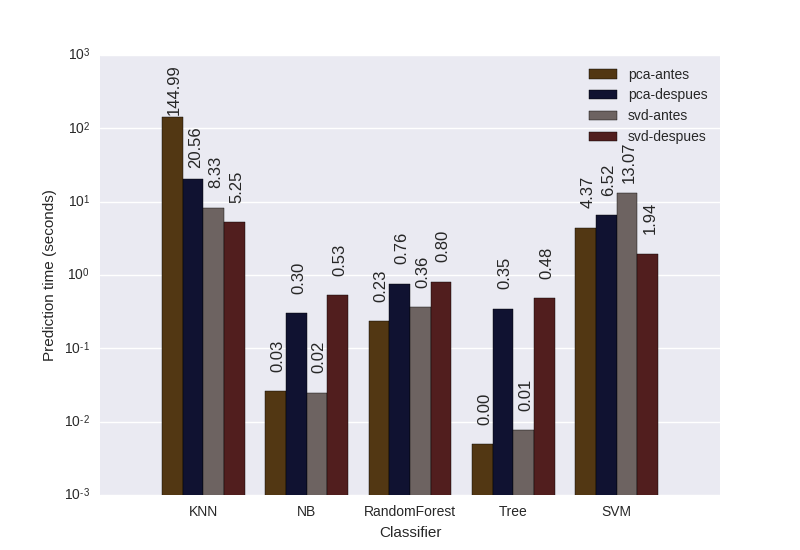
\includegraphics[width=1\textwidth]{../results/tiempos.png}
	\caption{Tiempo de clasificación de una muestra de 18000 emails de los distintos clasificadores en escala logarítmica.}
	\label{figure:time}
\end{figure}

Los gráficos de las Figuras \ref{figure:precision} y \ref{figure:accuracy} permiten analizar una gran variedad de propiedades sobre los clasificadores. Como primer punto, nuestra hipótesis de querer forzar a utilizar algunas features agregándolas luego de aplicar la reducción de dimensionalidad, parecería no estar justificado en el caso de PCA, no solo no mejora, sino que la performance del clasificador es mayor si dejamos que PCA realice esta tarea. Lo dicho anteriormente parece no aplicar a SVD en el caso de accuracy (Figura \ref{figure:accuracy}), donde la performance agregando nuestras features posteriormente (svd-despues) mejora notablemente respecto de SVD agregando nuestras fuatures antes (svd-antes). Creemos que esto se debe a que en el proceso de reducción de dimensionalidad, SVD descarta una parte importante de las features que determinamos y que contienen mucha información importante para la clasificación.
Como segundo punto podemos confirmar, por suerte, que medir el accuracy al entrenar no representó una caída en la performance al contrastar con los datos de test. Esto lo vemos justificado, como mencionamos en la sección anterior, a que las clases spam y ham están balanceadas.
También podemos ver que la performance de Random Forest es, coherentemente, muy similar a de árbol de decisión.
Algo peculiar que puede observarse en la Figura \ref{figure:precision} es que el \textit{precision} (minimizar falsos positivos) aumenta en todos los clasificadores respecto al \textit{accuracy} para el caso de realizar SVD sobre todas las features. Es decir, no forzar a utilizar ciertas features, parecería favorecer a disminuir este tipo de error.
Haciendo una evaluación sobre los tiempos que toma cada clasificador en evaluar el dataset separado para testing (Figura \ref{figure:time}), parecería no estar justificado elegir SVM o KNN por sobre Random Forest, que tiene un tiempo de corrida significativamente más rápido y obtiene además la mejor performance. Hay que destacar que por cuestiones de tiempos, no pudimos efectuar \textit{grid-seach} de forma extensiva para SVM, por lo cual no sabemos cuanto podría mejorar con una configuración más óptima de parámetros.

